\section{Domínio de aplicação do sistema}

Com o diagrama abaixo representado (Figura~\ref{fig:2}) é possível visualizar todos os atores do software 
e as suas ações, assim como também os sistemas envolvidos na aplicação e as suas funções.
Destes é possível identificar que este software contém três atores principais, o Utilizador que é um 
utilizador sem sessão iniciada, o Técnico que é um utilizador com sessão iniciada, já a Empresa é uma empresa
cliente da Motorline. Também é possível visualizar os diferentes sistemas integrados no 
projeto, como Servidor Motorline onde serão obtidas informações de catálogo de produtos, 
Servidor Install \& Go onde estão todas as funções de suporte ao software, o Servidor de Imagens onde 
serão guardadas todas as imagens do fórum e por fim o Servidor de Email que enviará email com o código de 
validação de conta para os clientes assim que se registarem no software .

\begin{figure}[htb]
    \centering
    
    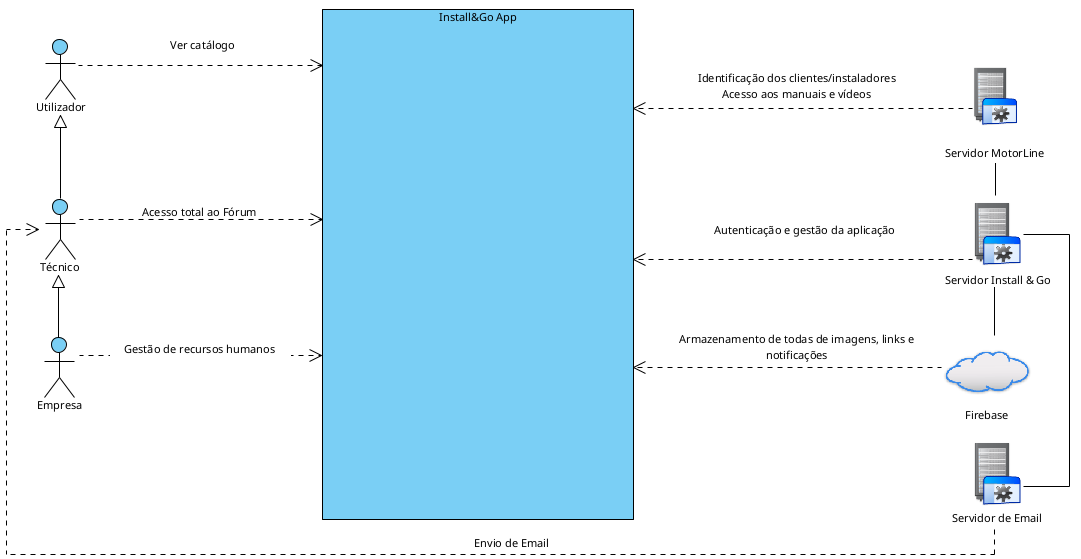
\includegraphics[width=\textwidth]{images/diagramas/diagrama_contexto.png}
    \caption{Diagrama de contexto da aplicação}
    \label{fig:2}
\end{figure}
